%\documentclass{sigchi}
\documentclass{article}



\usepackage{graphics} % for EPS, load graphicx instead
\begin{document}


\title{HabilisX: Document Exploration Through a Tool-Based Touch Screen Environment }
\author{Prairie Rose Goodwin}
\date{}
\maketitle
\begin{abstract}
This project explores a new touch screen interface for interacting with data sets through a digital tool metaphor.  Research in psychology has shown that when we hold a tool, such as a hammer, our minds frame potential solutions around the affordances of the tool.  Additionally, metaphors have proven to be a powerful way to positively affect user experience, in part because the user has expectations about how different objects behave.  Our system attempts to recreate the experience of using physical tools. Touch screens provide the ideal interaction style for this metaphor because they allow the user to be more physically engaged than a traditional point-and-click interaction. With the support of the James B. Hunt Library at North Carolina State University, we created a work environment with life-size tools using a 40-inch PixelSense 2.0 touch screen table.  Our interface consists of two and a half dimensional representations of paperclips, pushpins, rulers, magnifying glasses, "magic lenses", and sticky notes that can be used to manipulate database entries that appear as index cards scattered randomly on the table.  All objects on the screen have physical properties like center of mass, momentum, and friction to mimic the behavior of real objects on a table.  The tools are designed to let the user search and organize the data efficiently by taking advantage of spatial cognition and information visualizations.  Moreover, the user can leverage basic filtering queries by attaching "filter tiles" to the tools that dictate the entries with which the tools will interact.  Our goal is to show that our system is user-friendly and allows users to categorize data faster and more accurately than a comparable tabular interface.
\end{abstract}
\section{keywords}


\section{Introduction}	

%Tool use is a fundamental aspect of the ways in which humans interact with their environments, bot in the physical world and within the computer interface. 
%
%Analogies in software environments follow naturally from our experience with tools in the real world.  
%
%The ubiquity and effectiveness of the tool metaphor in software environments suggest that people's experiences with everyday physical tools carries over to the use of software tools.  Yet little effort has been put into understanding the characteristics of physical tool use and how those characteristics may support or undermine interactions when adapted to software design.
%
%We believe that an improved understanding of the nature of tool use and its related concepts can help us to generate better explanations of why many software tools are effective.  Further, the application of these concepts can lead to the development of novel interaction techniques.  
%
%The separation between physical and cognitive tool use is not a sharp line;  
%
%
%The applications in this section illustrate how tools can influence design in domains that may  have less than obvious physical interpretations.
\section{Related Work} 
\subsection{Tool Metaphor}

GUI Metaphors allow users to represent problems in a more easily solvable format.  As cognitive tools defined by Hutchins \cite{Hutchins1995} and Norman \cite{Norman1991}, they have shown that they can be extremely powerful aids.  Since the introduction of the desktop metaphor by Xerox in the '70's  it has become ubiquitous for personal computers.  Command line usability is notoriously difficult for beginners and non-technical users, whereas being able to interact with visual icons gives users an underlying model of what their actions are doing.  This allowed a whole new demographic to use computers, and subsequently the adoption of home computers skyrocketed.  

This project explores a novel user interface with a tool metaphor for database searches.  Tool metaphors have been introduced at a surface level in some conventional software environments.  Most notably visual programs like photoshop or paint have a tools that have analogs to real world objects.  However, the metaphor is usually quite shallow, and beyond icon and task, bear little resemblance to the experience of using that tool.  This is important because there is a cognitive shift that occurs when using a physical tool in which the user starts to think of the tool as an extension of his or her body.  \cite{Maravita2004}  When we factor in the affordance of a tool, we realized that tool metaphors have the ability to remold the experience into something familiar.  

Direct manipulation interfaces provide a good environment to explore affordances in software \cite{Gaver1991}, \cite{Norman1991}.  Users interact directly with objects on the screen instead of with menus or commands \cite{Hutchins1989} \cite{Shneiderman1992}, which are continuously represented with animation instead of appearing and disappearing as needed.\cite{Shneiderman1992}  Getner argued that deeper metaphors that are more consistent with the physical world can improve learnability and usability of the system \cite{Gentner1996} and can be a good opportunity for the user to become familiar with the system \cite{Fischer1994}.  


\subsection{Spatial Cognition}
There is a large body of work that has shown the cognitive benefits of being able to organize items spatially. \cite{Agarawala2006} \cite{Robertson1998} Robertson et al. made a 2½-D interface for bookmarking website that showed dramatic improvement in efficiency and error over the built in text-based system.  
	
	Most work has been done between a graphical environment versus a textual environment, but Sebrechts et al took this concept one step further and did a formal evaluation of a text-based, 2-D, and 3-D interfaces.\cite{Sebrechts1999}  They found that the 2-D interface had the best performance in both user satisfaction and performance.  Additionally, they tried multiple input devices, which made a significant impact on the usability of the interface. 

\subsection{Touch}
Touch screens have become popular in recent years, but many feel that they are a step backwards in usability \cite{Norman2010}.  Gestures have many of the drawbacks of a command line interface: commands can be hard to remember, impossible to explore, and hard to debug.  There are no visual cues for what gestures the system will recognize, and there is not a standard set of gestures for all functionality.   Some work has been done to standardize gestur

 
	New work suggests that multi-touch interfaces may also have a usability gain for expert users when used appropriately.  \cite{Forlines2007} \cite{Tan2002}\cite{North2009}.  Multi-touch is more efficient in the amount of time to select targets than the mouse.  Moreover, when you can get full embodied interaction that comes with large touch screens, more cognitive benefits can be seen. Kinesthetic input has been shown to improve spatial memory. \cite{Tan2002}.  Tan et. All found a 19\% increase in spatial recall in an experiment document retrieval setting.  

\cite{North2009}
North et. al have classified gestures on surfaces for a selection task of 2D objects with the number of hands used and the number of items in a group.

\cite{Forlines2007}
Previous research has compared traditional indirect-
Mapping input devices such as a mouse with MT devices. For
example, Shanis et. al [14] tested MT against mouse and 
touchpad for speed, performance and wrist posture. They 
showed that cursor positioning was better with the mouse 
and that MT caused significantly less wrist extension than 
the touchpad, but was comparable to the mouse. Forlines et 
al. [2] have shown that MT is more efficient (i.e., less time) 
than mouse in target selection, but worse in shape 
matching. Wigdor et al measured accuracy of the Ripples 
MT system with traditional target selection tasks [6]. 
Overall, researchers have compared the MT t the mouse in 
the face of traditional computer tasks, such as single target 
acquisition and shape dragging.	

The results of two 
experiments show that for bimanual tasks performed on 
tabletops, users benefit from direct-touch input. However, 
our results also indicate that mouse input may be more 
appropriate for a single user working on tabletop tasks 
requiring only single-point interaction.
\cite{Kristensson2008}
Thus our user study indicates that multi-touch can act as a useful complementary interaction method in information visualization interfaces.



\subsection{Large Displays}
\cite{Darken1996}
\cite{Ball2007}
\cite{Czerwinski2003}
\subsection{Document Management}
\cite{Bier2005}
\cite{Foo2007:ICADL}
\cite{Mothe1998}
\cite{Newman2010}
\cite{Nowell1996}
\cite{schraefel2002}
\cite{Shneiderman2000}
\cite{Yost2006}

\section{Habilis}


Our system has a well established set of interaction mechanisms, and clear parallels to physical tools in the real world.

We propose a novel way to display and organize information visually through the metaphor of physical tools. Tool-use in the physical world generally includes an object in the operator's hand and broad motions to perform an action. We propose to extend these concepts to digital tools by implementing a program on the Microsoft Pixelsense 2.0 that lets the user select (pick-up) tools on the screen and perform motions that mimic physical tool usage. 
Program description:

\begin{figure}[t!]
\centering
\scalebox{.239}
{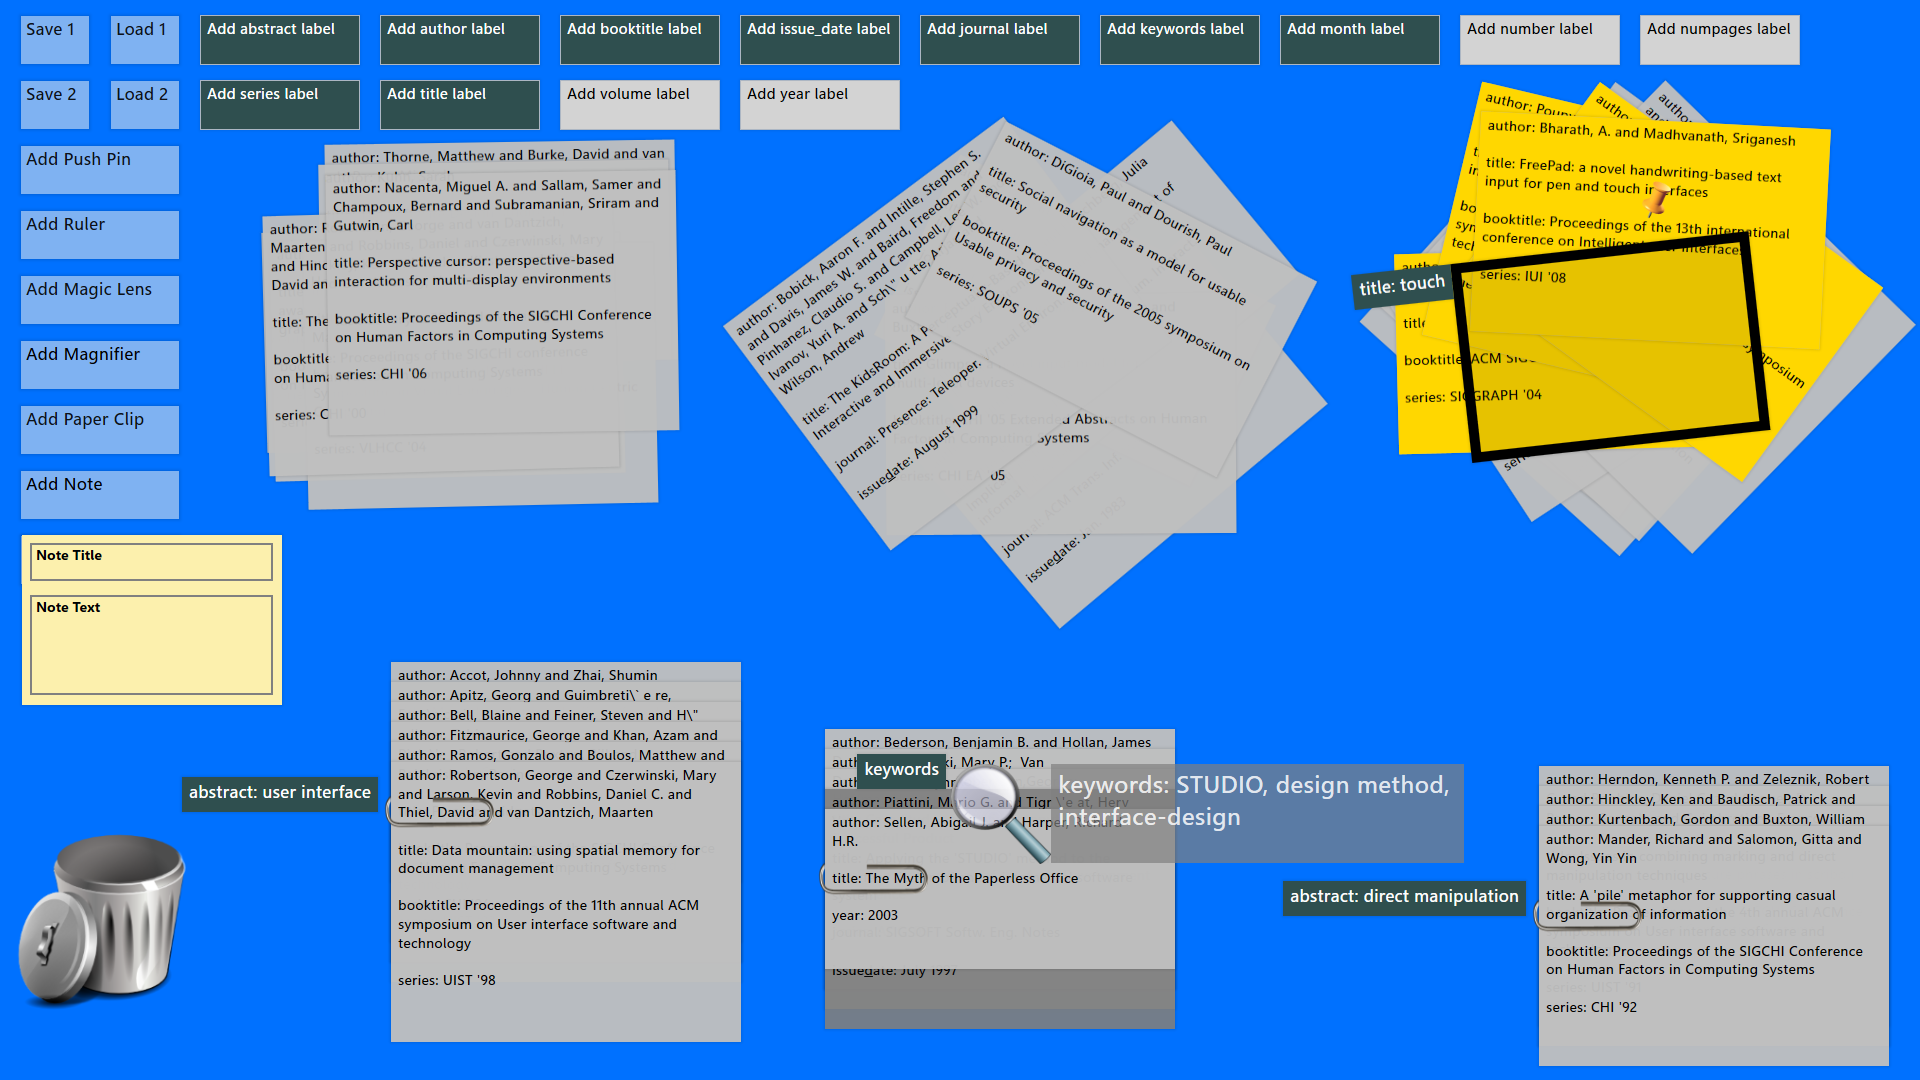
\includegraphics{HabilisScreenShot.png}}
\caption{Screenshot of Habilis after having used all tools.}
\label{Fig:screenshot}
\end{figure}



This program would be used to search and organize information stored in a database.  After getting an initial body of entries to search, each entry will appear as individual tiles with properties of naive physics that can be moved around the screen by touch. 






\subsection{Save States}
Habilis included two save states.  You can switch between two configurations of data for comparative purposes.  The tools do not change when a save state is loaded.  This is in part to maintain object permanence, but also so that the same queries can be used on either configuration.  

\subsection{Filter Tiles}
The name of each attribute or column header is shown on buttons that generate a label when pressed. These labels specify search criteria and can be attached to the tools to determine the items with which the tool will interact. For example, if the attribute is a string, the user should be able to specify a particular string to search for. If the attribute is an int, the user should be able to use any of the compare functions available such as greater than, less than, etc. 

Example: Let's say that your data set is a collection of research papers with the attributes: 

(String) Title
(String) Author
(Date object) DatePublished
(List<String>) Keywords
(int) pages

If you are looking for a paper on computer vision published in the last 5 years that is between 5 and 10 pages, you could create the query labels:
\begin{itemize}
\item Pages: $>$ 5
\item Pages: $<$ 10
\item Date: $<$ 2000
\item Keywords: "Computer Vision"

\end{itemize}

A single tool that has all of these queries would match to a paper that is 5-10 pages long, published before the year 2000, with the author- supplied keyword "Computer Vision".


Once created, you can attach and detach the query labels to tools by intersecting the two objects to quickly interact with your data.

\subsection*{Sticky Note}
Sticky Notes attach directly to entries and look similar to a filter with a different background color.  Once attached, the note will display the title, but tap it once to switch to the body of the note, and again to see the title again.
\subsection{Habilis Tools}
Not all tools can accept filters.  The focus of this project was searching, so the tools that were useful for that task cab accept filters. However, for other tasks, we found it was more useful to have tools that were consistent for all entries.  These tools were used for modifying entries based on their location rather than their content.   	
\subsection*{Push Pin}
The pushpin is used to "save" entries.  Once pinned, the entry is immobilized and no other tool can modify that entry.  Entries can be thrown under a pin to create a messy pile.  
\subsection*{Ruler}
The ruler can push entries around the screen and organize them visually by aligning them horizontally or vertically.  This state is somewhere in between a tidy pile and a messy pile as it does not afford browsing.  However, it unmistakably shows you entries that are categorized together.  
\subsection*{Trash Can}
The trashcan removes any unwanted entries or tools.  Just like in a Desktop GUI, just drag the item to the trash can, and it will disappear from the screen.  
\subsection{Habilis Filter Tools}
The following tools can be modified by attaching filter tiles.  Once attached, the tool will only interact with the entries that match the tile's query.  
\subsection*{Magic Lens}
The magic lens is a window that highlights entries that match your query.  Additionally, the lens will pop the results to the front of the interface so that no result is hidden.  
\subsection*{Magnifier}
The magnifier lets you view any attribute of an entry.  Simply drag the filter tile to the magnifier and instead of creating a query, the corresponding data of that attribute will be displayed in a pop-up next to the tool.  Drag any number of filter tiles, and the attribute will be displayed below the last one.  
\subsection*{Paper Clip}
Paper clips are used to create organized piles, or "tidy piles".  If no filters are attached, the paper clip will pick up everything.  If a filter tile is added, it will drop any entries that do not mach the query.  
%\subsection{Metaphor Structures}
%\subsection*{Messy Piles}
%\subsection*{Tidy Piles}
%like piles
\subsection{Habilis Interaction Design}
The buttons that were initially placed on the screen to populate the tools are not movable, scalable, or rotatable.  They can be activated by a quick or long touch and have no other interactions.  

All other UI Elements were sub-classed from a ScatterViewItem and have the same interaction properties.  All elements have have physical properties like center of mass, momentum, and friction to mimic the behavior of real objects on a table.  You can drag them around using one finger, but having two fingers on the tool disabled its use so that you could drag it around the screen without interactions with other UI elements.  

Once a filter tile or note has been attached to its target, it can be removed with a long touch (1.5 seconds).  
\section{User Study}
\subsection{Methods}
\subsection*{Subjects}
	Eight Computer Science graduate students between the ages of 22 to 26 from various research specialties participated in this study.  No one had previous experience using Habilis or the SUR40, while six out of eight had no previous experience with Mendeley. All subjects were male with  normal or corrected-to-normal vision with no other known disabilities. 
\subsection*{Equipment}
	Habilis was run on the Samsung SUR40 40-inch touch screen table with no external hardware.  Users were forced to use only touch interactions with a virtual onscreen keyboard. Mendeley was run on a Sony Flip-PC touch screen convertible laptop.  However, no user chose to utilize the touch interactions of the laptop, and instead used a wireless mouse and build in keyboard.  
	
\subsection*{Procedure}

	This experiment was a comparative study between Habilis and Mendeley.  To test which system was better for organizing documents into categories, users were asked to identify citations of a source paper.  We chose to use Bumptop \cite{Agarawala2006}
	as our source paper because it has many sources that neatly divide into several subjects.  The authors also released a seven minute video that gives a detailed overview of all of the features and novel designs without mentioning their sources.   
	
	Bumptop had forty-one sources that encompassed six subjects: advantages of a pile metaphor, stylus interactions, spacial organization, realism, browsing techniques, naive physics, and animation.  Dataset 1 encompassed twenty-one papers covering pile metaphors, stylus interactions, and spacial organization.  The remaining twenty papers went into dataset 2.  Distractor papers were added from mobile and touchscreen research until each dataset had a total of thirty-seven papers.  The subjects were then asked to identify which papers were related to bumptop.  The datasets were alternated between Habilis and Mendeley to overcome any performance bias of the data.  The trials were timed, and at the end they were asked 3 questions:
	\begin{enumerate}
	\item Which system did you prefer? why?
	\item Did you see any topic clusters?  If so, what topics?
	\item What features were you looking for but didn't see in Habilis?
	\end{enumerate}
\section{Results}
\subsection*{Performance Time}
\subsection*{Number of Incorrect Categorizations}
%\subsection*{Failed Trials}
%Table of Questionaire
\section{Discussion \& Future Work}

%\subsection{''subsection''}	2	not in letters
%\subsubsection{''subsubsection''}	3	not in letters

\bibliographystyle{plain}
%\bibliographystyle{acm-sigchi}
\bibliography{890}{}
\end{document}
